\documentclass[a4paper,11pt]{article}
\usepackage[utf8]{inputenc}
\usepackage{amsmath}
\usepackage{amsfonts}
\usepackage{amssymb}
\usepackage{graphicx}

\numberwithin{equation}{section}
\renewcommand\thesubsection{\alph{subsection}}
\newcommand{\bvp}[1]{\mathbf{#1}'}
\newcommand{\bv}[1]{\mathbf{#1}}
\newcommand{\pp}[1]{#1'}


%opening
\title{Thesis Proposal: Separating Cyclostationary Signals using the Nonlinear Dynamics of Continuous-Time Recurrent Networks}
\author{Vince Baker}

\begin{document}

\maketitle

\section{Abstract}
Recurrent, continuous-time networks have powerful computational properties. \\
Liquid state machines with high dimensional nonlinear dynamics are a biologically plausible mechanism for cognitive tasks. \\
Nonlinear delay dynamics can virtualize spatial nodes into temporal time slots. \\
Ultrafast photonic implementation can virtualize very large spatial networks that run at slower timescales. \\
Many signals of interest are stationary or cyclostationary.\\
Spike-timing dependent plasticity is a plausible biological mechanism for liquid state network training.\\



\section{Introduction} 

\section{Thesis Statement}

\section{Approach}
Use a recurrent network of nodes with a range of time scales as a near-chaotic resevoir.
Model the networks using apprpriate tools (NEURON, MATLAB ODE, Keras).
Investigate biologically plausible connectivities and determine the onset of the chaotic regime.
Train the readout to recognize cyclostationary signals using a biologically plausible mechanism such as spike-time-dependent plasticity.


\section{Preliminary results}

\section{Work plan}
\begin{figure}
 \caption{Schedule}
 \centering
   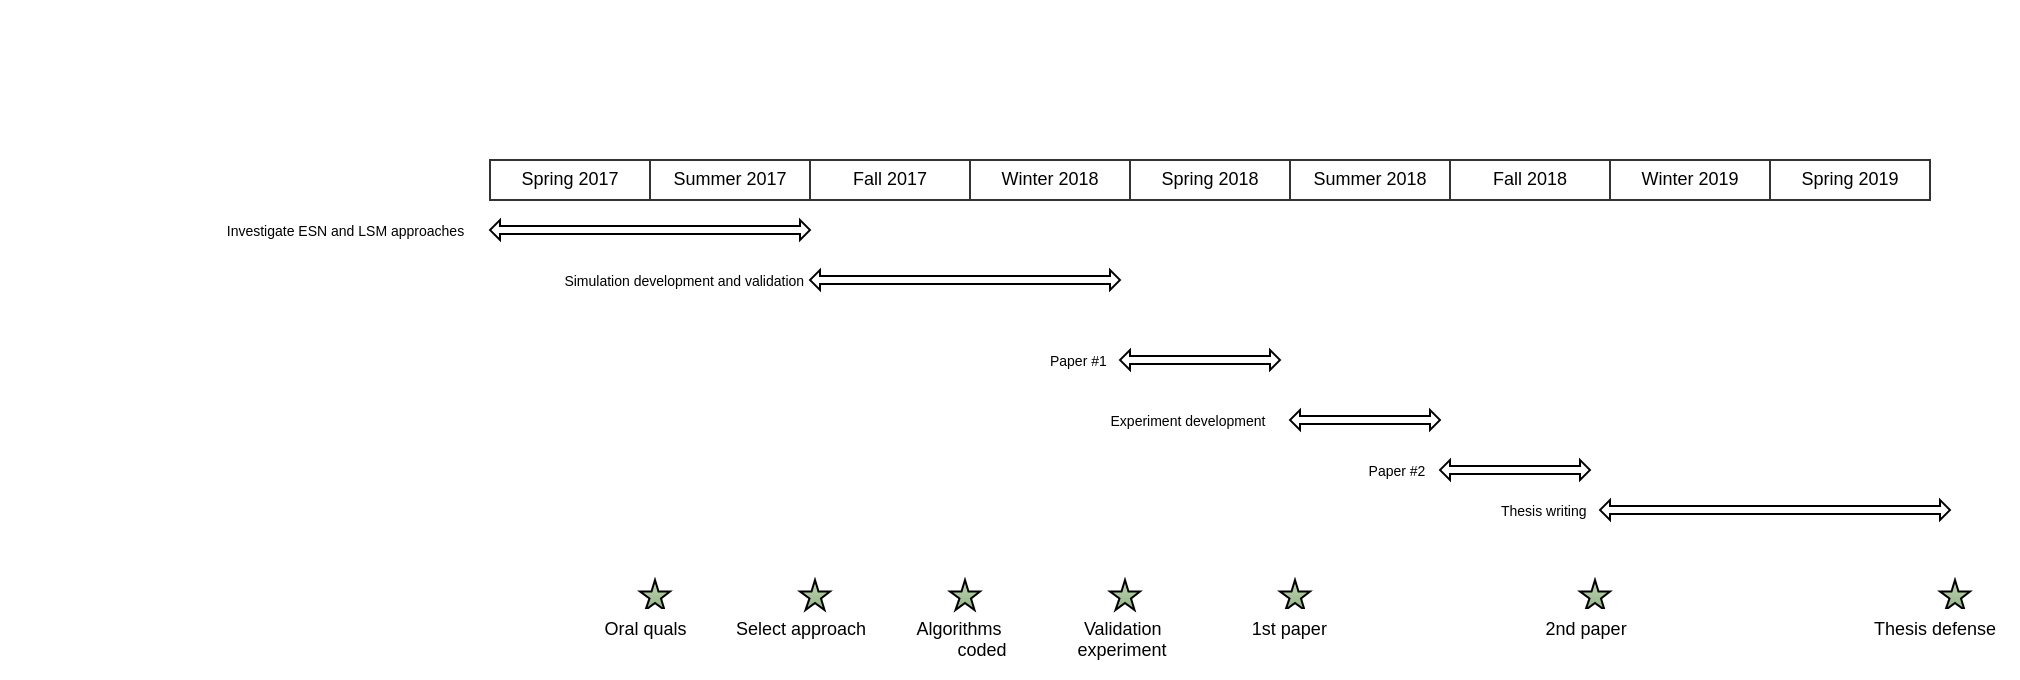
\includegraphics[width=\textwidth]{ThesisSchedule}
\end{figure}

\section{Implications of research}

\section{References}

\end{document}
